
%% bare_jrnl.tex
%% V1.4b
%% 2015/08/26
%% by Michael Shell
%% see http://www.michaelshell.org/
%% for current contact information.
%%
%% This is a skeleton file demonstrating the use of IEEEtran.cls
%% (requires IEEEtran.cls version 1.8b or later) with an IEEE
%% journal paper.
%%
%% Support sites:
%% http://www.michaelshell.org/tex/ieeetran/
%% http://www.ctan.org/pkg/ieeetran
%% and
%% http://www.ieee.org/

%%*************************************************************************
%% Legal Notice:
%% This code is offered as-is without any warranty either expressed or
%% implied; without even the implied warranty of MERCHANTABILITY or
%% FITNESS FOR A PARTICULAR PURPOSE! 
%% User assumes all risk.
%% In no event shall the IEEE or any contributor to this code be liable for
%% any damages or losses, including, but not limited to, incidental,
%% consequential, or any other damages, resulting from the use or misuse
%% of any information contained here.
%%
%% All comments are the opinions of their respective authors and are not
%% necessarily endorsed by the IEEE.
%%
%% This work is distributed under the LaTeX Project Public License (LPPL)
%% ( http://www.latex-project.org/ ) version 1.3, and may be freely used,
%% distributed and modified. A copy of the LPPL, version 1.3, is included
%% in the base LaTeX documentation of all distributions of LaTeX released
%% 2003/12/01 or later.
%% Retain all contribution notices and credits.
%% ** Modified files should be clearly indicated as such, including  **
%% ** renaming them and changing author support contact information. **
%%*************************************************************************


% *** Authors should verify (and, if needed, correct) their LaTeX system  ***
% *** with the testflow diagnostic prior to trusting their LaTeX platform ***
% *** with production work. The IEEE's font choices and paper sizes can   ***
% *** trigger bugs that do not appear when using other class files.       ***                          ***
% The testflow support page is at:
% http://www.michaelshell.org/tex/testflow/

\documentclass[10pt,journal,compsoc]{IEEEtran}
%
% If IEEEtran.cls has not been installed into the LaTeX system files,
% manually specify the path to it like:
% \documentclass[journal]{../sty/IEEEtran}



% *** CITATION PACKAGES ***
%
%\ifCLASSOPTIONcompsoc
  % IEEE Computer Society needs nocompress option
  % requires cite.sty v4.0 or later (November 2003)
  \usepackage[nocompress]{cite}

% *** GRAPHICS RELATED PACKAGES ***
\usepackage{graphicx}
\graphicspath{ {./images/} }


% *** MATH PACKAGES ***
%
\usepackage{amsmath}
% A popular package from the American Mathematical Society that provides
% many useful and powerful commands for dealing with mathematics.
%
% Note that the amsmath package sets \interdisplaylinepenalty to 10000
% thus preventing page breaks from occurring within multiline equations. Use:
%\interdisplaylinepenalty=2500
% after loading amsmath to restore such page breaks as IEEEtran.cls normally
% does. amsmath.sty is already installed on most LaTeX systems. The latest
% version and documentation can be obtained at:
% http://www.ctan.org/pkg/amsmath



% *** SPECIALIZED LIST PACKAGES ***
%
%\usepackage{algorithm,algorithmic}
\usepackage[ruled]{algorithm2e}
% algorithmic.sty was written by Peter Williams and Rogerio Brito.
% This package provides an algorithmic environment fo describing algorithms.
% You can use the algorithmic environment in-text or within a figure
% environment to provide for a floating algorithm. Do NOT use the algorithm
% floating environment provided by algorithm.sty (by the same authors) or
% algorithm2e.sty (by Christophe Fiorio) as the IEEE does not use dedicated
% algorithm float types and packages that provide these will not provide
% correct IEEE style captions. The latest version and documentation of
% algorithmic.sty can be obtained at:
% http://www.ctan.org/pkg/algorithms
% Also of interest may be the (relatively newer and more customizable)
% algorithmicx.sty package by Szasz Janos:
% http://www.ctan.org/pkg/algorithmicx




% *** ALIGNMENT PACKAGES ***
%
\usepackage{array}
% Frank Mittelbach's and David Carlisle's array.sty patches and improves
% the standard LaTeX2e array and tabular environments to provide better
% appearance and additional user controls. As the default LaTeX2e table
% generation code is lacking to the point of almost being broken with
% respect to the quality of the end results, all users are strongly
% advised to use an enhanced (at the very least that provided by array.sty)
% set of table tools. array.sty is already installed on most systems. The
% latest version and documentation can be obtained at:
% http://www.ctan.org/pkg/array


% *** SUBFIGURE PACKAGES ***
%\ifCLASSOPTIONcompsoc
%  \usepackage[caption=false,font=normalsize,labelfont=sf,textfont=sf]{subfig}
%\else
  \usepackage[caption=false,font=footnotesize]{subfig}
%\fi
% subfig.sty, written by Steven Douglas Cochran, is the modern replacement
% for subfigure.sty, the latter of which is no longer maintained and is
% incompatible with some LaTeX packages including fixltx2e. However,
% subfig.sty requires and automatically loads Axel Sommerfeldt's caption.sty
% which will override IEEEtran.cls' handling of captions and this will result
% in non-IEEE style figure/table captions. To prevent this problem, be sure
% and invoke subfig.sty's "caption=false" package option (available since
% subfig.sty version 1.3, 2005/06/28) as this is will preserve IEEEtran.cls
% handling of captions.
% Note that the Computer Society format requires a larger sans serif font
% than the serif footnote size font used in traditional IEEE formatting
% and thus the need to invoke different subfig.sty package options depending
% on whether compsoc mode has been enabled.


% *** PDF, URL AND HYPERLINK PACKAGES ***
%
\usepackage{url}
% url.sty was written by Donald Arseneau. It provides better support for
% handling and breaking URLs. url.sty is already installed on most LaTeX
% systems. The latest version and documentation can be obtained at:
% http://www.ctan.org/pkg/url
% Basically, \url{my_url_here}.




% *** Do not adjust lengths that control margins, column widths, etc. ***
% *** Do not use packages that alter fonts (such as pslatex).         ***
% There should be no need to do such things with IEEEtran.cls V1.6 and later.
% (Unless specifically asked to do so by the journal or conference you plan
% to submit to, of course. )

%Alessandro input: makecell package to permite line break inside tables
\usepackage{makecell}
\usepackage{xcolor}

% correct bad hyphenation here
\hyphenation{op-tical net-works semi-conduc-tor}

%\renewcommand{\baselinestretch}{0.975}

\begin{document}
%
% paper title
% Titles are generally capitalized except for words such as a, an, and, as,
% at, but, by, for, in, nor, of, on, or, the, to and up, which are usually
% not capitalized unless they are the first or last word of the title.
% Linebreaks \\ can be used within to get better formatting as desired.
% Do not put math or special symbols in the title.
%\title{Building a framework to perform automated verification of solar photovoltaic off-grid systems}
\title{Multi-core synthesis and maximum satisfiability applied to obtain optimal sizing of solar photovoltaic systems}
%
%
% author names and IEEE memberships
% note positions of commas and nonbreaking spaces ( ~ ) LaTeX will not break
% a structure at a ~ so this keeps an author's name from being broken across
% two lines.
% use \thanks{} to gain access to the first footnote area
% a separate \thanks must be used for each paragraph as LaTeX2e's \thanks
% was not built to handle multiple paragraphs
%

\author{Alessandro~Trindade, Edilson Galvão and Lucas~Cordeiro% <-this % stops a space
\IEEEcompsocitemizethanks{
\IEEEcompsocthanksitem{A. Trindade is with the Department of Electricity, Federal University of Amazonas, Manaus, Brazil, e-mail: alessandrotrindade@ufam.edu.br.}% <-this % stops a space
\IEEEcompsocthanksitem{E. Galvão is with ???, Manaus, Brazil, e-mail: esj.galvao@gmail.com.}
\IEEEcompsocthanksitem{L. Cordeiro is with School of Computer Science, The University of Manchester, UK, e-mail: lucas.cordeiro@manchester.ac.uk.}}% <-this % stops a space
\thanks{The authors would like to thank ????, for the financial support.}
\thanks{Manuscript received november 23, 2020; revised XXXXX 11, 2020.}}

% note the % following the last \IEEEmembership and also \thanks - 
% these prevent an unwanted space from occurring between the last author name
% and the end of the author line. i.e., if you had this:
% 
% \author{....lastname \thanks{...} \thanks{...} }
%                     ^------------^------------^----Do not want these spaces!
%
% a space would be appended to the last name and could cause every name on that
% line to be shifted left slightly. This is one of those "LaTeX things". For
% instance, "\textbf{A} \textbf{B}" will typeset as "A B" not "AB". To get
% "AB" then you have to do: "\textbf{A}\textbf{B}"
% \thanks is no different in this regard, so shield the last } of each \thanks
% that ends a line with a % and do not let a space in before the next \thanks.
% Spaces after \IEEEmembership other than the last one are OK (and needed) as
% you are supposed to have spaces between the names. For what it is worth,
% this is a minor point as most people would not even notice if the said evil
% space somehow managed to creep in.



% The paper headers
\markboth{IEEE Transactions on Computers,~Vol.~XX, No.~YY, January~2021}%
{Trindade \MakeLowercase{\textit{et al.}}: Multi-core synthesis and maximum satisfiability applied to obtain optimal sizing of solar photovoltaic systems}
% The only time the second header will appear is for the odd numbered pages
% after the title page when using the twoside option.
% 
% *** Note that you probably will NOT want to include the author's ***
% *** name in the headers of peer review papers.                   ***
% You can use \ifCLASSOPTIONpeerreview for conditional compilation here if
% you desire.




% If you want to put a publisher's ID mark on the page you can do it like
% this:
%\IEEEpubid{0000--0000/00\$00.00~\copyright~2015 IEEE}
% Remember, if you use this you must call \IEEEpubidadjcol in the second
% column for its text to clear the IEEEpubid mark.



% use for special paper notices
%\IEEEspecialpapernotice{(Invited Paper)}






% As a general rule, do not put math, special symbols or citations
% in the abstract or keywords.
\IEEEtitleabstractindextext{%
\begin{abstract}
(IEEE TOSE text, not published yet)There exist various methods and tools to size solar photovoltaic systems; however, these tools rely on simulations, which do not cover all aspects of the design space during the search for the optimal solution. In prior studies in optimal sizing, the focus was always on criteria or objectives. Here, we present a new sound and complete approach to obtaining optimal sizing using an unprecedented program synthesis technique. Our variant of counterexample guided inductive synthesis (CEGIS) approach has two phases linking the technical and cost analysis. First, we synthesize a feasible candidate based on power reliability, but that may not achieve the lowest cost. Second, the candidate is then verified iteratively with a lower bound cost via symbolic model checking. If the verification step does not fail, the lower bound is adjusted; and if it fails, a counterexample provides the optimal solution. Experimental results using seven case studies and commercial equipment data show that our synthesis method can produce within an acceptable run-time the optimal system sizing. We also compare our approach with a commercial tool specialized in photovoltaic systems optimization. Both results are validated with commercial design software to show the effectiveness of our approach.
(VSTTE) In the current scenario, energy demand rises by 1.3\% each year to 2040, and photovoltaic (PV) systems have emerged as an alternative to the fossil or nuclear fuel energy generation. The use of formal methods for PV systems is a new subject with significant research spanning only five years. Here we develop and evaluate  an automated synthesis technique to obtain optimal sizing of PV systems based on Life Cycle Cost (LCC) analysis. The optimal solution is the lowest cost from a list of equipment that meets the electrical demands from a house, plus the replacement, operation, and maintenance costs over $20$ years. We propose a variant of the counterexample guided inductive synthesis (CEGIS) approach with two phases linking the technical and cost analysis to obtain the PV sizing optimization. We advocate that our technique has various advantages if compared to off-the-shelf optimization tools available in the market for PV systems. Experimental results from seven case studies demonstrate that we can produce an optimal solution within an acceptable run-time; different software verifiers are evaluated to check performance and soundness. We also compare our approach with a commercial tool specialized in PV systems optimization. Both results are validated with commercial design software; furthermore, some real PV systems comparison are used to show our approach effectiveness.
\end{abstract}

% Note that keywords are not normally used for peerreview papers.
\begin{IEEEkeywords}
Formal synthesis, software verification, model checking, solar photovoltaic systems.
\end{IEEEkeywords}}

% make the title area
\maketitle

% For peer review papers, you can put extra information on the cover
% page as needed:
% \ifCLASSOPTIONpeerreview
% \begin{center} \bfseries EDICS Category: 3-BBND \end{center}
% \fi
%
% For peerreview papers, this IEEEtran command inserts a page break and
% creates the second title. It will be ignored for other modes.
\IEEEpeerreviewmaketitle



\IEEEraisesectionheading{\section{Introduction}}
% The very first letter is a 2 line initial drop letter followed
% by the rest of the first word in caps.
% 
% form to use if the first word consists of a single letter:
% \IEEEPARstart{A}{demo} file is ....
% 
% form to use if you need the single drop letter followed by
% normal text (unknown if ever used by the IEEE):
% \IEEEPARstart{A}{}demo file is ....
% 
% Some journals put the first two words in caps:
% \IEEEPARstart{T}{his demo} file is ....
% 
% Here we have the typical use of a "T" for an initial drop letter
% and "HIS" in caps to complete the first word.
--------------------
\color{blue} 
\IEEEPARstart{T}{he} recent studies about global energy indicate that 789 million people have no access to electricity, which is 10\% of the world population~\cite{Energyprogressreport}. From 2010 until 2018 the effort to reduce the number of people without access to electricity increased and the result was positive. Quantitatively the result was a decrease from 1.2 billion to 0.84 billion people without electrical energy, of this total, renewable energy solutions are responsible for 136 million people receiving basic energy service~\cite{Energyprogressreport}. Unfortunately, lack of access to clean and affordable energy is considered a core dimension of poverty~\cite{Hussein2012} and this has a direct impact on the low HDI (Human Development Index) of different localities~\cite{Coelho}. It follows that increased access to energy allows economic growth and poverty alleviation\cite{Karekesi}. 

To provide electricity for all, decentralized systems led by solar photovoltaic (PV) in off-grid and mini-grid systems will be the lowest-cost solution for three-quarters of the connections needed~\cite{Hussein2012}. Thus, this can be ratified by analyzing the result of renewable energy reported by global bank, where 17.3\%  of global energy is based on wind and solar energy~\cite{Energyprogressreport}.

In front of world changes to improve the electrical energy uses, The more precise the dimensioning for electrical networks, the more effective the use of renewable energies. For this purpose, there are some software available in the market, a part of them is created to general purpose like MATLAB~\cite{Benatiallah2017} and others for specific energy study like RETScreen, and HOMER~\cite{Pradhan,Swarnkar}. However, the
industry demands the design solution to be the optimum, considering equipment manufacturers and models available on the market and not just minimum or maximum
values of current or power for the optimized items. We need to evaluate the electrical compatibility among the equipment, which can only be achieved with specialized PV optimization software. Therefore, the optimal solution is the
lowest cost from a list of equipment that meets the house’s electrical demands.
\color{black}

Here, we have developed a variant of counterexample guided inductive synthesis (CEGIS)~\cite{AbateCAV2018} for synthesizing optimal sizing of stand-alone PV systems using commercial equipment data. If the user gives a correctness specification $\sigma$, our method uses that as a starting point and then iteratively produces a sequence of candidate solutions that satisfy $\sigma$, related to power reliability.


\color{blue} 
In this tool, we used a solver called Z3. Internally, the Z3 tool contains a module to include optimization objectives, this module is named vZ and integrates state-of-the-art algorithms for optimization and extra tools to solve linear restrictions problems. In particular, the vZ features match our problem and will help us to optimize PV systems~\cite{BjornerPF15}.
In particular, in each iteration, we synthesize the sizing of stand-alone PV systems, but that may not achieve the lowest cost. Thus, the candidate solution passes through an SMT solver to reduce the number of possible states, a lower bound is provided by our candidate solution, which serves as the minimum cost of reference will help our engine in restrictions verification; Note, each iteration can be cost lower or higher than current reference, once found a value lower than the current reference, and it respects the user constraints, the reference is updated globally. 
If the verification step does not fail, all content produced is saved as a counterexample with an optimal sizing that meets both power reliability and system cost. If the verification step does fail, the content produced is ignored. Our novelty relies on a practical approach to the pursuit of the optimal solution of PV systems using formal methods. 

\color{red} aqui precisas mudar este parágrafo para que reflita a nova técnica que estamos usando, citando paralelismo multi-core e o solver vZ que é dedicado para otimização\color{black}
%Our work makes two major contributions. \textbf{First}, the use of automated symbolic verification methods in electrical systems was rare in recent prior studies~\cite{abs-1811-09438}, and specifically their use in synthesizing optimal PV sizing is unprecedented. Here, a list of PV components (i.e., PV panels, charge controllers, inverters, and batteries) can be fed to our proposed synthesis method together with user requirements and environment constraints, and our synthesis algorithm based on symbolic model checking can find the optimal solution in technical and economical terms. \textbf{Second}, %our experimental results show that our synthesis method is an effective and efficient approach on the pursuit of the optimal solution of PV systems using formal methods, which outperforms existing state-of-the-art simulation tool. As a result, 

\color{blue} In summary, this paper makes the following original contributions: (i) It is an radical improvement in terms of performance of the first use of formal synthesis for stand-alone PV systems  application~\cite{VSTTE2020}, which provides accurate and detailed results of optimal sizing of stand-alone PV systems. (ii) We propose a variant CEGIS method with striking differences of how the SYNTHESIZE and VERIFY phases work together, with the suppression of the feasible solution candidate vector and the use of a parallel loop to reach the optimal cost solution of the system. (iii) Experimental results with seven case studies show that the formal synthesis approach qualitatively outperforms an existing state-of-the-art optimization tool. Our solution is completely detailed and closer to commercial reality (real PV systems). The results are validated with accurate commercial design software called PVsyst
\color{black}

%\textit{Contribution}. Our study marks the first application of a sound and automated formal synthesis approach that can provide accurate results of optimal sizing of stand-alone PV systems, which outperforms an existing state-of-the-art simulation tool used in a comparative with seven case studies. In particular, the methodological research with automated synthesis produces more detailed and complete optimization when compared with the simulation tool, besides the fact that the sizing is closer to real PV systems deployed at isolated communities in the Amazon area of Brazil. Considering other studies carried out in the last two decades, we considerably advance the state-of-the-art in applied energy to optimally design PV systems.
%\textit{Outline}. Section~\ref{sec:Background} gives the background about sizing and optimization of PV systems. Section~\ref{sec:Method} presents the automated formal synthesis proposed in this underlying study. Section~\ref{sec:Results} is devoted to the experimental evaluation, while Section~\ref{sec:Conclusion} presents the conclusions and describes future work.

%-----------------------------------------------------------
\section{Background}
\label{sec:AutomatedVerification}
%-----------------------------------------------------------
\vspace{-1ex}\color{blue}
Fig.~\ref{fig:optimization} illustrates how to obtain the optimal sizing of a stand-alone PV system using two different modes, the first one is the traditional model called \textit{\textbf{traditional sizing}} that include manual verification, which means calculus about electrical equipment capacity and installation for validation. Allied to the first mode, there are still commercial tools like MATLAB~\cite{Benatiallah2017} and Homer~\cite{Pradhan,Swarnkar} to try to simulate the real electrical system. The second and on the opposite side, the model well-knows as \textbf{\textit{Automated Synthesis}} that encompasses BMC engines. This option proves to be more powerful since it generates more complex and accurate data than the traditional way described previously.
Both modes described here use the same input and theoretically tend to produce the same output, it is noteworthy that variables such as electrification, support for different categories of equipment and different forms of electrical dimensioning, impact on the expected output.

For \textbf{Input} data, we can consider weather data, price information about each equipment, design requirements, load curve, power demand, and design assumptions. This information is converted programmatically into a matrix of data and exposed as global content to the software. For \textbf{Output} data, the major information denotes that renewable energy systems can be combined(price and system hardware composition), when it occurs, the answer of the system need be SAT. Otherwise, the answer of the system is UNSAT.
%
\begin{figure}[h]
\fbox{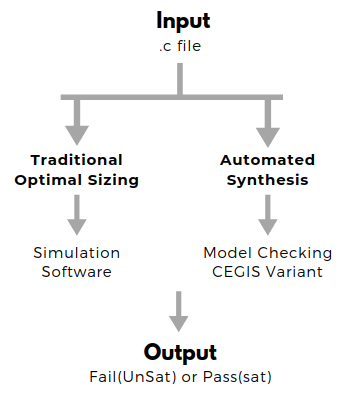
\includegraphics[width=0.38\textwidth]{TraditonalVsAutoFlow.png}}
\centering
\caption{Comparative image of the traditional method versus the proposed method.}
\label{fig:optimization}
\end{figure}

\color{blue}
The automated synthesis technique is mathematical reasoning about a model, where the result is a rich counterexample that has detailed information on the optimal solution, thus, the answer can guide the software or client to choose the best combination of electrical machines. Contrariwise, the traditional way don't offer the quantity of necessary data about the system and internal modes. Another special topic that needs to hightlighted is about coverage of each model, models that use automated kernel can to assurance a complete coverage overall state space, instead of, locals states as a traditional model. 

\color{black}


%-----------------------------------------------------------
\subsection{Program Synthesis}
\label{sec:ProgramSynthesis}
%-----------------------------------------------------------
The basic idea of program synthesis is to automatically construct a $ P $ program that satisfies a correctness specification $\sigma$. In particular, program synthesis is automatically performed by engines that use a correctness specification $\sigma$, as a starting point, and then incrementally produce a sequence of candidate solutions that partially satisfy $\sigma$~\cite{Abateetal2017}. As a result, a given candidate program $p$ is iteratively refined to match $\sigma$ more closely. Figure~\ref{Counter-Example-Guided-Inductive-Synthesis} illustrates the underlying architecture. 
%
\begin{figure}[h]
\begin{center}
\fbox{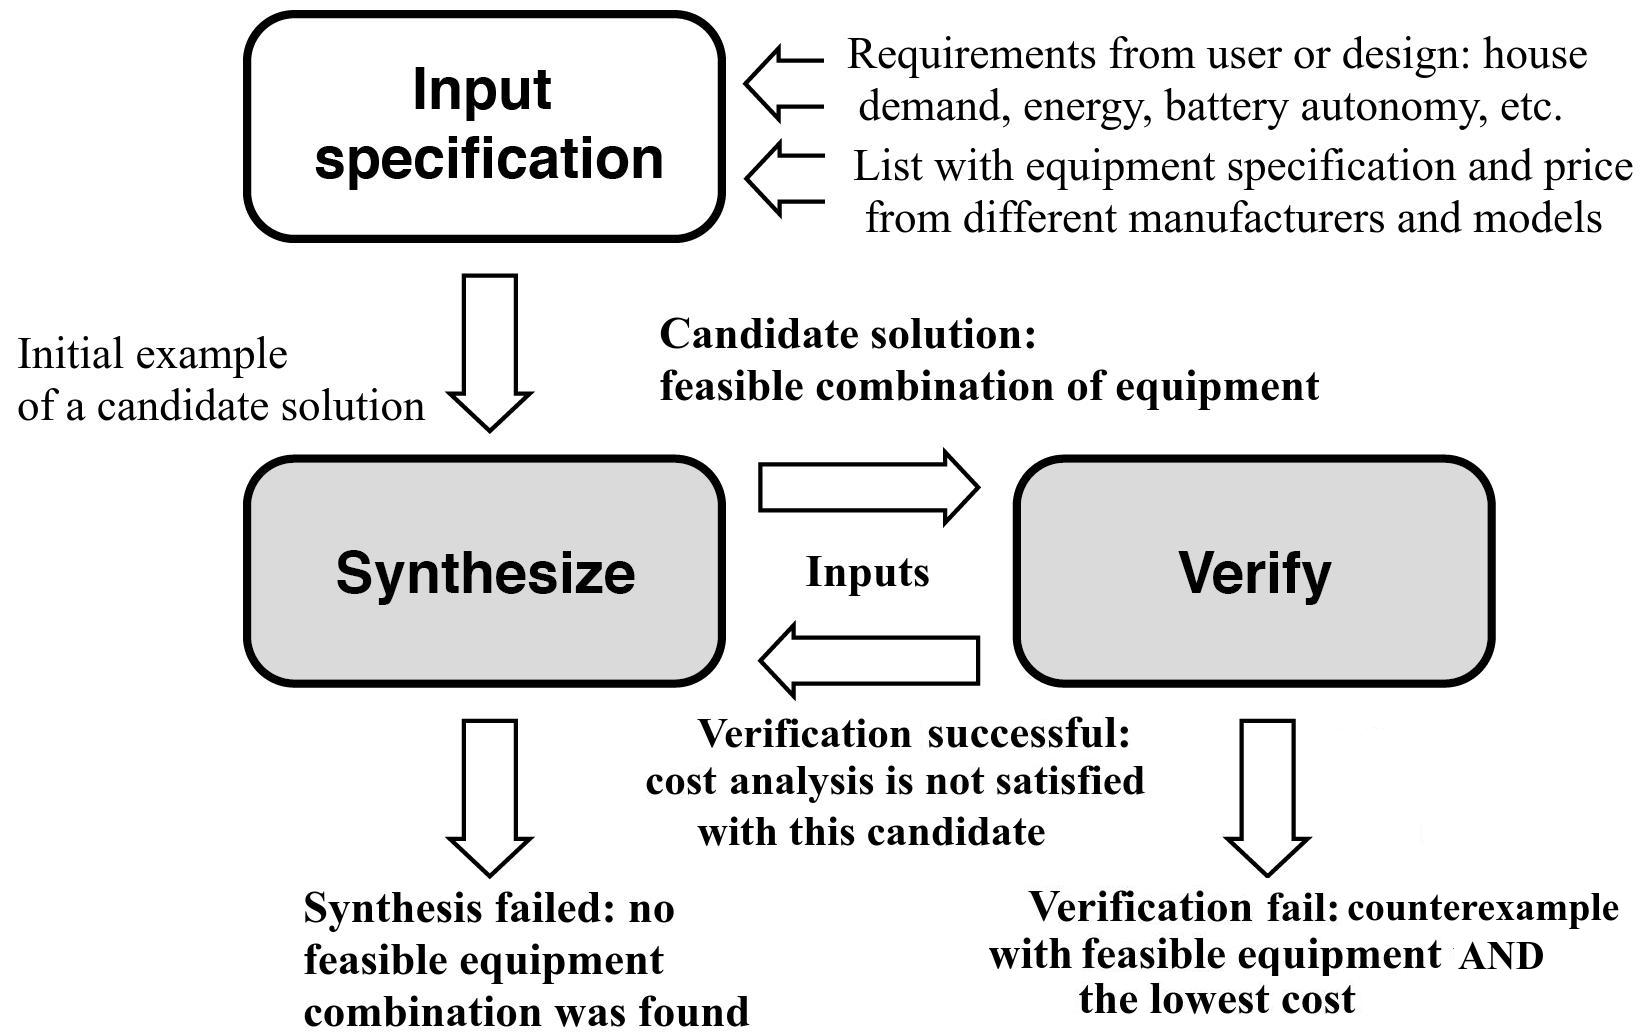
\includegraphics[width=0.47\textwidth]{fig2_rev2.jpg}}
\end{center}
	\caption{CEGIS in PV system sizing.}
	\label{Counter-Example-Guided-Inductive-Synthesis}
\end{figure}

The correctness specification $\sigma$ provided to our synthesizer is of the form $\exists \vec{F}. \forall \vec{x}. \sigma(\vec{x}, \vec{F})$, where $\vec{F}$ ranges over functions, $\vec{x}$ ranges over ground terms, and $\sigma$ is a quantifier-free (QF) formula typically supported by SMT solvers. The ground terms are interpreted over some finite domain $\mathcal{D}$, where $\mathcal{D}$ can be encoded using the SMT's bit-vectors part. Our specification includes house demand, energy, and battery autonomy; we also provide equipment specifications and prices from different manufacturers and models.

In Figure~\ref{Counter-Example-Guided-Inductive-Synthesis}, the phases {\sc Synthesize} and {\sc Verify} interact via a finite set of test vectors {\sc inputs}, which is incrementally updated. Given the correctness specification $\sigma$, the {\sc Synthesize} procedure tries to find an existential witness $\vec{F}$ satisfying the specification $\sigma(\vec{x}, \vec{F})$, for all $\vec{x}$ in {\sc inputs} (as opposed to all $\vec{x} \in \mathcal{D}$). If {\sc Synthesize} succeeds in finding a witness~$\vec{F}$, the latter is a candidate solution to the full synthesis formula, which is passed to {\sc Verify} to check whether it is a proper solution ({\it i.e.}, $\vec{F}$ satisfies the specification $\sigma(\vec{x}, \vec{F})$ for all $\vec{x}\in\mathcal{D}$). If this is the case, then the algorithm terminates.

One may notice that each iteration of the traditional CEGIS loop adds a new input to the finite set $INPUTS$, which is then used for synthesis. Given that the full set of inputs $\mathcal{D}$ is finite because we use bit-vector expressions, the refinement loop can only iterate over a finite number of times. However, {\sc Synthesize} may conclude that no candidate solution obeying $\sigma$ for the finite set $INPUTS$ exists. 

In our CEGIS variant, there exist four differences related to the traditional one: 
(1) there exists no test vector, and every candidate is generated in the {\sc Synthesize} phase and sent to the {\sc Verify} phase; 
(2) if the {\sc Verify} phase is unsuccessful, then a new candidate is generated by {\sc Synthesize} and 
(3) the lower bound of the {\sc Verify} phase is incremented to search for the lowest cost; as a result,
(4) there exists no refinement from the {\sc Verify} phase back to the {\sc Synthesize} phase. In particular, a new counterexample is not added to the {\sc input} set since a failure during the {\sc Verify} phase will only discard a given candidate, which could be feasible in the next iteration with a new lower bound.

In summary, our proposal is a technique based on CEGIS, which aims to synthesize the optimal solution of a PV system; therefore, our technique addresses an optimization problem.

%%%%%%%%%%%%%%%%%%%%%%%%%%%%%%%%%%%%%%%%%%%%%%%%%%%%%%%%
\subsection{Sizing Stand-alone Solar PV Systems}
\label{sec:sizing}
%%%%%%%%%%%%%%%%%%%%%%%%%%%%%%%%%%%%%%%%%%%%%%%%%%%%%%%%

A PV system is illustrated in Fig.\ref{fig:blockdiagram}. It employs the PV generator (\textit{panel or an array}), a semiconductor device that can convert solar energy into DC electricity. For night hours or rainy days, we hold \textit{batteries}, where power can be stored and used. The use of batteries as a storage form implies the presence of a \textit{charge controller}~\cite{Hansen}. The PV arrays produce DC, and therefore when the PV system contains an AC load, a DC/AC conversion is required (\textit{inverter}). The \textit{AC load} dictates the behavior of the AC electrical load from the house that will be fed by the system.
%
\begin{figure}[h]
\fbox{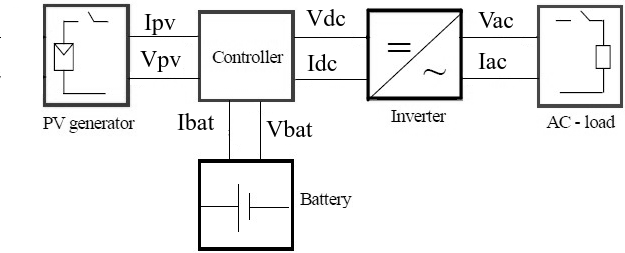
\includegraphics[width=0.47\textwidth]{blockdiagramPVS2_rev}}
\centering
\caption{Block diagram for a typical stand-alone PV system~\cite{Hansen}.}
\label{fig:blockdiagram} 
\end{figure}

The sizing check stage can ensure that the system meets the standard project steps related to the critical period method (worst month) for solar energy system sizing~\cite{Pinho}. It adopts an MPPT (Maximum Power Point Tracking) charge controller, which is the most common in use. 

Since this paper's audience is targeted to be from the software verification area, we decided to use a higher-level explanation about the PV sizing. The sizing process involves a set of eighteen equations related to the electrical engineering area, which is detailed online.\footnote{\url{https://tinyurl.com/yck7dfxt}} Fig.~\ref{fig:flow} illustrates the overview of the steps that must be taken to size a stand-alone PV system.
%
\begin{figure}[h]
\fbox{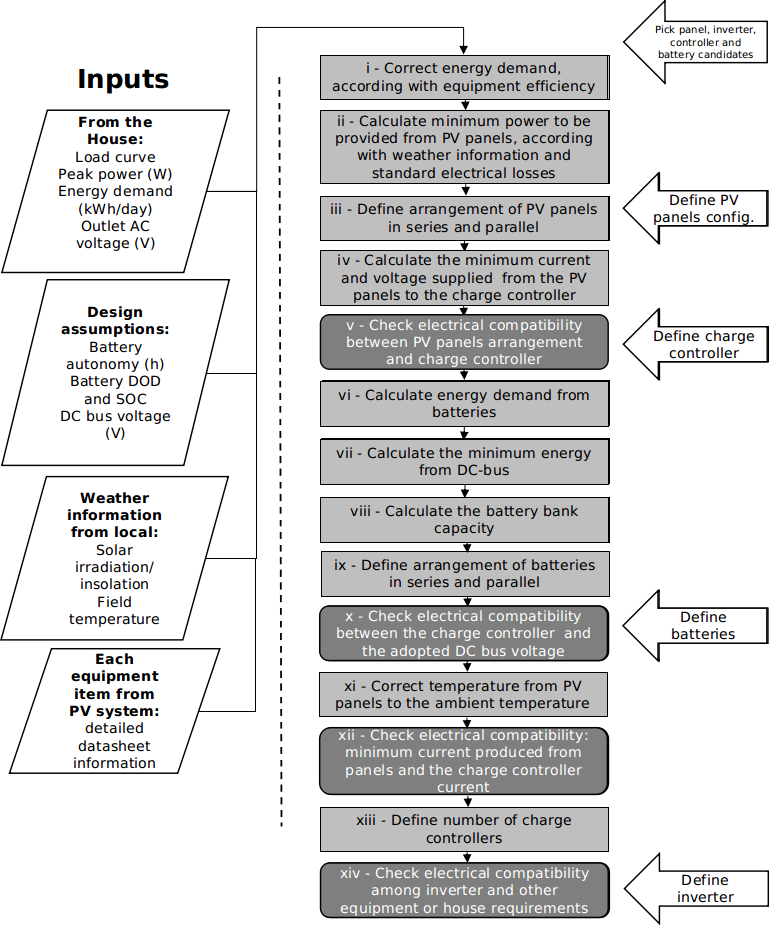
\includegraphics[width=0.47\textwidth]{flowchart}}
\centering
\caption{High level description of stand-alone PV system sizing process.}
\label{fig:flow} 
\end{figure}

On the left side of Fig.~\ref{fig:flow}, we describe the needed \textbf{inputs} to size a PV system. There exist requirements from the house to be electrified; in particular, we have the design assumptions, weather information from the targeted local of the PV system deployment, and a possible initial list of equipment to be used, covering all the items listed in Fig.\ref{fig:blockdiagram}. Concerning the equipment list, the designer can use a few pieces of equipment or a vast one. We can also decide not to adopt the commercial equipment list. However, the result is a PV sizing of specific power, current, or voltage values, and usually just close to original equipment, which can be found in the market. This possibility has the drawback of possible incompatibility among equipment when the real one is bought and deployed.

There exist specific steps that aim the calculation of some variables and others related to the electrical compatibility validation among equipment items, both enumerated from \textbf{i} to \textbf{xiv}, as illustrated in Fig.~\ref{fig:flow}; those represent different shades of gray of the rectangle boxes. The start point is usually a candidate list of PV panels, charge controller, battery, and inverter, as indicated at the top of the flowchart. The arrows, on the right side, show a point where some specific item is validated. The diagram does not show the returning location. However, if the candidate item is not compatible with others or does not meet some requirement, it must be changed to follow the indicated flow. The last rectangle box checks the inverter electrical compatibility with the DC-bus voltage, with the required AC voltage from the outlet. Besides, the inverter specified power must be lower than the charge controller power to avoid it from burning by overcharge. At the end of the flowchart, all the items are defined, and the PV sizing is finished.

These equations model the continuous-time behavior of the PV system; they produce real numbers except for the batteries and panels, where real numbers must be converted into integer ones, considering the minimum or maximum according to each equation. The verification and simulation tools need to handle non-linear real arithmetic to produce the correct result. Our mathematical model uses floating-point arithmetic. It is just an approximation of the real numbers. However, in this work, we are not concerned with calculating the rounding error, which is negligible when considering the size of the physical quantities and the variables adopted~\cite{DBLP:journals/corr/abs-2004-12699}.

%------------------------------------------------------
\section{Synthesizing Optimal Sizing of Stand-alone Solar Photovoltaic Systems}
%------------------------------------------------------

The best compromise between two objectives makes the optimal sizing of PV systems: \textit{power reliability} and \textit{system cost}~\cite{Alsadi2018}. This study will rely on the critical period solar energy method~\cite{Pinho}, as described in Section~\ref{sec:sizing}. Our study will use an adapted Life Cycle Cost (LCC) analysis, where the acquisition cost of every item of equipment is considered, plus the installation cost, the operational and maintenance costs~\cite{Alsadi2018}, given as,
%
\begin{equation}
\label{eq:LCC}
LCC = C_{PV} + C_{bat} + C_{charger} + C_{inv} + C_{installation} + C_{batrep} + C_{PWO\&M}
\end{equation}

\noindent where $C_{PV}$ is the PV array cost, $C_{bat}$ is the initial cost of batteries, $C_{charger}$ is the cost of the charger, $C_{inv}$ is the inverter cost, $C_{installation}$ is the installation cost, $C_{batrep}$ is battery replacement cost at current prices, and $C_{PWO\&M}$ is operation and maintenance costs at current rates. In this study, we will use a $C_{installation}$ equivalent to 5\% of total equipment cost and a $C_{PWO\&M}$ equal to U\$ 289.64/year according to Amazon State literature data~\cite{Agrener2013}; and a LCC lifetime analysis of 20 years.

\color{blue} In this section, we will describe a couple of pseudo-code that embassy our tool and how model checking was used as a backend verification engine~\cite{DBLP:journals/corr/abs-1909-13139}. The Algorithm~\ref{base_opt_code} describes how to save and expose the correct solutions and the optimal solution, and Algorithm~\ref{base_opt_code2} is responsible to verify the mathematical assertion over electrical equipaments.\\

\color{red} à partir daqui tu usas várias vezes a palavra \textbf{node}, mas em nenhum lugar tu explicas o que é. Se é uma árvore de busca então creio que precisas explicar o que é (na seção background) para poder falar agora no algoritmo em si\color{blue}

\begin{algorithm}[h]
\SetAlgoLined
\KwResult{returns a feasible sizing of PV system with the lowest cost}
%returns the lowest possible cost with the best configuration of photovoltaic equipment.}
Initialize arrays and variables\;
Create Satisfable List called \textit{NodeSatList}\;
Create maximumCost as a long variable\;
\ForAll {AllAvailableNodes node}
{%
    isLowestNode = solve(node)\\
     \If{$\var{isLowestNode} = true$}
     {
        lock(this)\\
        maximumCost = node.cost \\
        NodeSatList.add(node)\\
        unlock(this)\\
    }
}
\textbf {return} NodeSatList.OrderBy(x.Cost).FirstOrDefault()
\caption{Find by the optimal solution}
\label{base_opt_code}
\end{algorithm}

Algorithm~\ref{base_opt_code} is started based in input described on Fig.~\ref{fig:optimization}, it contemplate manufacturer’s data, prices of PV panels, batteries, charge controllers, and inverters. Programmatically this set of data are represented in arrays and global variables, which have the purpose of assisting the storage of counterexamples and the maximum possible cost. Moreover, we define design (house) requirements and design assumptions to help backend solvers. The parallel loop is used to process each node separately, the function \textit{solve} that will described in Algorithm~\ref{base_opt_code2} returns true when the node is a possible solution and the cost is lower than global maximum cost. Therefore, to assure the correct storage of result processed by many threads at same time, the lock function was added. After the internal loop ends, the last action returns the optimal solution found in the list that contains all possible solutions.\\

\begin{algorithm}[h]
\SetAlgoLined
\KwResult{Verify if the node is satisfactory for restrictions and equipment.}
Initialize internal arrays and variables\;
\SetKwProg{Fn}{Function}{:}{}
  \Fn{\FMain{$solve(node)$}}{
\textbf{Step 01.} Declare non-deterministic variables to select PV Panel, Controller, Battery, and Inverter from list \\
\textbf{Step 02.} Calculate Steps i and ii of Fig.~\ref{fig:flow} \\
\textbf{Step 03.} Define PV panels arrangement: Step iii of Fig.~\ref{fig:flow} \\
\textbf{Step 04.} Calculate Step iv of Fig.~\ref{fig:flow} \\
\textbf{Step 05.} Enforce electrical compatibility in Step v of Fig.~\ref{fig:flow} with statement \textbf{assume} \\
\textbf{Step 06.} Calculate Steps vi to viii of Fig.~\ref{fig:flow} \\
\textbf{Step 07.} Define battery arrangement according Step ix of Fig.~\ref{fig:flow} \\
\textbf{Step 08.} Enforce electrical compatibility in Step x of Fig.~\ref{fig:flow} with statement \textbf{assume} \\
\textbf{Step 09.} Correct variables to ambient temperature: Step xi of Fig.~\ref{fig:flow} \\
\textbf{Step 10.} Enforce electrical compatibility in Step xii of Fig.~\ref{fig:flow} with statement \textbf{assume} \\
\textbf{Step 11.} Define number of charge controllers: Step xiii of Fig.~\ref{fig:flow}\\
\textbf{Step 12.} Enforce electrical compatibilities in Step xiv of Fig.~\ref{fig:flow} with statement \textbf{assume} and define the inverter \\
\textbf{Step 13.} Non-deterministic variables hold feasible equipment and cost \\
$F_{obj} \leftarrow N_{TP}*Panel_{Cost} \, + \, N_{TB}*Battery_{Cost} \, + Controller_{Cost} \, + \, Inverter_{Cost} \, + \, Installation_{Cost} \, + \, batrep_{Cost} \, + \, PWO\&M_{Cost}$ \\
\KwRet\ isSatisfiable;
  }
\caption{Verify if the node is satisfactory for restrictions and equipment.}
\label{base_opt_code2}
\end{algorithm}

To choose the best option, the system uses as input a
list of \textbf{seventy} equipment from \textbf{twelve} different manufacturers, where each technical information required was found in a datasheet provided by the equipment factory). To calculate equation~\ref{eq:LCC} value it was necessary to convert the amounts to US dollars based on the exchange rate of the day. To simplify understanding about this type of data, a report has created that condensates general information required to perform tests over this tool, and it is available online.\footnote{\url{https://tinyurl.com/ycgbsgkp}}

The Algorithm 2 recover the information described above based on arguments provided by ”solve” function and creates an internal context. This context is responsible to check if all equation is satiable, at this moment all ”assume” marks that contain the constraints are added.

The pseudocode contains three points to be attention: The first point is the set of equations that correspond to a valid combination of electrical components. These equations can be found at steps 02, 03, 04, 06, 07, 09, 11 and 13. The second point refers to all four "assume" function is necessary because it serves as a limit or barrier of acceptable values to equipments. These restrictions can be found at steps 05, 08, 10 and 12, sequentially this steps represents battery bank, charge controller voltage check, does the inverter check and ensures the power demand and the surge power of the inverter. the last one point, the return system that can be SAT or UNSAT. The created context is saved in node variable and note that fobj described in last step is a cost of equipament.

The algorithm always returns two different states, SAT when the electrical equipaments combinations and the general cost are safe to became a possible solution and  UNSAT, once the program finishes without finding a solution, indicating that it was unable to combine the specific items of equipment to create a feasible solution. In some scenarios, you can expect a memory overflow or excessive time (timeout) resulting in a system with no concrete result, it is most common in hardware with few gigabytes of memory. The main challenge for the Algorithm~\ref{base_opt_code2} is to find a feasible candidate solution for the constraints and user requirements.

Summarizing: We use four non-deterministic variables
to index four matrices with complete datasheet information from an equipment item. We have four variables and four matrices: one to PV panels, one to batteries, one to the inverter, and one to the charge controller. Those nondeterministic variables are used during the search for the feasible solution and controlled by the statements assume. Note that the process described here is completely automated to ensure that the solution is sound. The verification engines transform the Algorithm~\ref{base_opt_code2} into the Boolean expressions that are passed to the solver to verify (C and !P), as described online.\footnote{\url{https://tinyurl.com/yajfmavl}}

\color{black}


%---------------------------------------------------------------------------
\section{Results and Discussion}
%---------------------------------------------------------------------------
%---------------------------------------------------------------------------
\subsection{Description of the Case Studies}
%---------------------------------------------------------------------------

The proposed synthesis approach was evaluated in seven stand-alone PV system case studies.
These case studies were defined based on the usual electrical load found in riverside communities in the Amazonas State, Brazil~\cite{TrindadeCordeiro19,Agrener2013}, except for case 7, which was idealized to support a few lamps and a 12k BTUs air-conditioner solution. 
Here we report each case study as a 4-tuple \textit{\{power peak (W); power surge (W); energy consumption (Wh/day); battery autonomy (hours)\}} as follows:
\textbf{1:} \{342; 342; 3,900; 48\}; \textbf{2:} \{814; 980; 4,880; 48\}; \textbf{3:} \{815; 980; 4,880; 12\}; \textbf{4:} \{253; 722; 3,600; 48\}; \textbf{5:} \{263; 732; 2,500; 48\}; \textbf{6:} \{322; 896; 4,300; 48\}; \textbf{7:} \{1,586; 2,900; 14,000; 48\}. This 4-tuple represents the Algorithm~\ref{alg:opt-algorithm} inputs. For all cases, an estimated load curve (kWh) was defined based on the electronics consumers in each house. Our synthesis algorithm was fed with data and costs of forty equipment items from ten different manufacturers of PV systems. 
%
Three state-of-the-art verifiers, CBMC\footnote{Command-line: \$ cbmc -\phantom{}-unwind 100 file.c -\phantom{}-trace} v5.11 with MiniSat 2.2.1~\cite{Kroening}, ESBMC\footnote{Command-line: \$ esbmc filename.c -\phantom{}-incremental-bmc -\phantom{}-boolector} v6.0.0~\cite{esbmc2018} with the Boolector 3.0.1 solver~\cite{Brummayer}, and CPAchecker\footnote{Command-line: \$ scripts/cpa.sh -heap 64000m -config config/bmc-incremental.properties -spec config/specification/sv-comp-reachability.spc file.c} v1.8~\cite{Beyer2011} with MathSAT 5.5.3~\cite{mathsat5}, were used as verification engines to compare the proposed approach effectiveness and efficiency. 

%---------------------------------------------------------------------------
\subsection{Optimization/Simulation Tools and Assumptions}
%---------------------------------------------------------------------------
Concerning the off-the-shelf optimization/simulation tools, only HOMER Pro performs an off-grid system with battery backup analysis and includes economical analysis. Here we used HOMER Pro version $3.13.1$ as a state-of-the-art optimization tool for comparison purposes. In particular, HOMER Pro has the following characteristics:
(a) it is available only for MS-Windows, its annual standard subscription costs US\$ $504.00$~\cite{HOMER}; 
(b) it has two optimization algorithms: one algorithm simulates all of the feasible system configurations defined by the search space, and additionally, a proprietary derivative-free algorithm to search for the least-costly system;
(c) it does not have LCC cost in its reports, only Net Present Cost (NPC); however, we can obtain LCC from NPC; 
(d) the optimization analysis defines a load curve and temperature according to data collected from online databases. However, to allow a correct comparison, the curve load and the temperature were defined the same as our synthesis approach; 
(e) it does not have a charge controller. During the tests, we have chosen the ``load-following'' option, which produces enough power to meet the demand~\cite{HOMER} and (usually) presents a non-overestimated solution; 
(f) it was assumed 95\% availability of the PV system. By definition, ``availability'' is the percentage of time at which a power system can feed the load requirements~\cite{Khatib2014}. For an ordinary house electrical load, 95\% is considered acceptable;
(g) it was assumed a string of two batteries to match the voltage of the $24$ V DC system, which was used for our automated synthesis tool; 
(h) it was included a generic flat-plate PV of $1$ kW and generic lead-acid batteries of $1$ kW ($83.4$ Ah capacity). During run-time, HOMER decides the size in kW of each one based on feasibility and lower cost.

To validate and compare the optimal sizing solution produced by our approach and by HOMER Pro, we use a simulation tool, called PVsyst version $6.86$~\cite{PVsyst}, with plenty of commercial equipment in its data bank. We have considered a comparison for an entire year's weather data of simulation to guarantee that the proposed sizing meets the electrification requirements. PVsyst is a PC software package developed by a Swiss company used for the study, sizing, simulation and data analysis of solar PV systems. PVsyst contains design, sizing, 3D shading scene, simulation, grid, and off-grid features. It uses comprehensive irradiation data from Meteonorm,\footnote{https://meteonorm.com/en/} and aging analysis~\cite{PVsyst2017}. However, it does not perform optimization; therefore, PVsyst needs the system sized to validate it. Furthermore, PVsyst does not have commercial inverter equipment and, as a result, does not consider surge power demand as the ones produced by air conditioners and refrigerators for a few seconds. PVsyst is commercial software with a $30$-day test possibility and runs only in MS-Windows.

%---------------------------------------------------------------------------
\subsection{Objectives and Setup}
%---------------------------------------------------------------------------

Our evaluation aims to answer three experimental goals: [EG1] \textbf{(soundness)} Does our automated synthesis approach provide correct results?; [EG2] \textbf{(performance)} How do the software verifiers compare to each other for synthesizing PV systems?; and [EG3] \textbf{(state-of-the-art)} how does our formal synthesis tool compare to a specialized simulation tool?

All experiments regarding the verification tools were conducted on an otherwise idle Intel Xeon CPU E5-4617 ($8$-cores) with $2.90$ GHz and $64$ GB RAM, running Ubuntu $16.04$ LTS $64$-bits. For HOMER Pro, we have used an Intel Core i5-$4210$ ($4$-cores) with $1.7$ GHz and $4$ GB RAM running Windows 10. The ideal scenario would be to use the same hardware configuration for the experiments. However, we faced restrictions concerning the license for the HOMER Pro tool; besides, we did not have the autonomy to change the Linux VM machine installed in our university's servers due to the internal policy. This setup has an impact on performance, which is less favorable to HOMER Pro. PVsyst used the same configuration as HOMER Pro. We perform the experiments with a predefined \textit{time out} of $660$ minutes.

%---------------------------------------------------------------------------
\subsection{Results}
%---------------------------------------------------------------------------

The results are presented in Table~\ref{tab1}. 
%
\begin{table*}
\centering
\caption{Case studies and results: optimization of stand-alone PV systems.}\label{tab1}
\begin{scriptsize}
\begin{tabular}{c|c|c|c|c}
\hline
\hline
Tools & \makecell{Microsoft Z3 \\(vZ 4.8.9)}& \makecell{ESBMC 6.0.0 \\(Boolector 3.0.1)}& \makecell{CPAchecker 1.8\\(MathSAT 5.5.3)}& HOMER Pro 3.13.1\\
\hline
\hline
Specification & Result & Result & Result & Result \\
\hline
\makecell{\textbf{Case Study 1}\\Peak:342W\\Surge:342W \\E:3,900Wh/day\\Autonomy:48h}&
\makecell{SAT (0,93 min) \\NTP:4$\times$()w\\NBT:8$\times$()Ah\\Controller 00A/000V\\Inverter 000W/0V\\LCC: US\$ 8,992.58} &
\makecell{SAT (620 min) \\NTP:6$\times$330W (2P-3S)\\NBT:16$\times$105Ah (2S-8P)\\Controller 35A/145V\\Inverter 700W/48V\\LCC: US\$ 10,214.04} & 
\makecell{SAT (548 min) \\NTP:6$\times$330W (2P-3S)\\NBT:16$\times$105Ah (2S-8P)\\Controller 35A/145V\\Inverter 700W/1600W/48V\\LCC: US\$ 10,214.04} & 
\makecell{(Time: 0.33 min)\\2.53 kW of PV\\NBT:12$\times$83.4Ah (2S-6P)\\0.351kW inverter\\LCC: US\$ 7,808.04}\\

\hline
\makecell{\textbf{Case Study 2}\\Peak:814W\\Surge:980W\\E:4,880Wh/day\\Autonomy:48h} & \makecell{SAT (0,42 min) \\NTP:6$\times$()w\\NBT:10$\times$()Ah\\Controller 00A/000V\\Inverter 000W/0V\\LCC: US\$ 10,028.34} &
TO &
TO &
\makecell{(Time: 0.18 min)\\3.71 kW of PV\\NBT:20$\times$83.4Ah (2S-10P)\\0.817kW inverter\\LCC: US\$ 12,861.75} \\

\hline
\makecell{\textbf{Case Study 3}\\Peak:815W\\Surge:980W\\E:4,880Wh/day\\Autonomy:12h} & \makecell{SAT (0,41 min) \\NTP:6$\times$()w\\NBT:10$\times$()Ah\\Controller 00A/000V\\Inverter 000W/0V\\LCC: US\$ 10,028.348} & 
\makecell{SAT (63 min) \\NTP:14$\times$150W (7P-2S)\\NBT:6$\times$105Ah (2S-3P)\\Controller 35A/145V\\Inverter 1,200W/48V\\LCC: US\$ 9,274.07} & TO & Not possible \\

\hline
\makecell{\textbf{Case Study 4}\\Peak:253W\\Surge:722W\\E:3,600Wh/day\\Autonomy:48h} & 
\makecell{SAT (0,72 min) \\NTP:4$\times$()w\\NBT:8$\times$()Ah\\Controller 00A/000V\\Inverter 000W/0V\\LCC: US\$ 8,883.62} &
\makecell{SAT (147 min) \\NTP:6$\times$330W (2P-3S)\\NBT:16$\times$105Ah (2S-8P)\\Controller 35A/145V\\Inverter 280W/48V\\LCC: US\$ 9,678.63} &
\makecell{SAT (605 min) \\NTP:6$\times$330W (2P-3S)\\NBT:16$\times$105Ah (2S-8P)\\Controller 35A/145V\\Inverter 280W/48V\\LCC: US\$ 9,678.63} &
\makecell{(Time: 0.23 min)\\2.42 kW of PV\\NBT:12$\times$83.4Ah (2S-6P)\\0.254kW inverter\\LCC: US\$ 7,677.95}\\

\hline
\makecell{\textbf{Case Study 5}\\Peak:263W\\Surge:732W\\E:2,500Wh/day\\Autonomy:48h} & 
\makecell{SAT (0,84 min) \\NTP:4$\times$()w\\NBT:6$\times$()Ah\\Controller 00A/000V\\Inverter 000W/0V\\LCC: US\$ 8,119.74} &
\makecell {SAT (36.70 min) \\NTP:4$\times$330W (2S-2P)\\NBT:14$\times$80Ah (2S-7P)\\Controller 35A/145V\\Inverter 280W/24V \\LCC: US\$ 8,900.70}
& \makecell {SAT (254.25 min) \\NTP:4$\times$330W (2S-2P)\\NBT:14$\times$80Ah (2S-7P)\\Controller 35A/145V\\Inverter 280W/24V \\LCC: US\$ 8,900.70} 
& \makecell{(Time: 0.18 min)\\1.59 kW of PV\\NBT:10$\times$83.4Ah (2S-5P)\\0.268kW inverter\\LCC: US\$ 6,175.57} \\

\hline
\makecell{\textbf{Case Study 6}\\Peak:322W\\Surge:896W\\E:4,300Wh/day\\Autonomy:48h} & 
\makecell{SAT (0,69 min) \\NTP:6$\times$()w\\NBT:10$\times$()Ah\\Controller 00A/000V\\Inverter 000W/0V\\LCC: US\$ 9,587.01} &
\makecell {SAT (380.93 min) \\NTP:6$\times$320W (2P-3S)\\NBT:18$\times$105Ah (2S-9P)\\Controller 35A/145V\\Inverter 400W/24V \\LCC: US\$ 10,136.61} & TO & \makecell{(Time: 0.22 min)\\3.15 kW of PV\\NBT:14$\times$83.4Ah (2S-7P)\\0.328kW inverter\\LCC: US\$ 9,112.45} \\

\hline
\makecell{\textbf{Case Study 7}\\Peak:1,586W\\Surge:2,900W\\E:14,000Wh/day\\Autonomy:48h} & \makecell{SAT (0,44 min) \\NTP:20$\times$()w\\NBT:30$\times$()Ah\\Controller 00A/000V\\Inverter 000W/0V\\LCC: US\$ 18,408.27}  &
UNSAT (0.48 min) & TO & \makecell{(Time: 0.20 min)\\12.5 kW of PV\\NBT:66$\times$83.4Ah (2S-33P)\\1.60kW inverter\\LCC: US\$ 41,878.11} \\
\hline
\hline
\end{tabular}
\\Legend: OM = out of memory; TO = time out; IF = internal failure; E = energy; NTP = total number of panels, NBtotal = total number of batteries, NPS = number of panels in series; NPP = number of panels in parallel, NBS = number of batteries in series; NBP = number of batteries in parallel; LCC = Life Cycle Cost.
\end{scriptsize}
\end{table*}
%
The violation (SAT result) indicated in Table~\ref{tab1} is the $assert$ of the line $18$ in Algorithm~\ref{alg:opt-algorithm} and suggests that an optimal solution was found.
Here, CBMC was unable to produce any conclusive result; \textit{out of memory} situations occurred in all case studies.

CPAchecker was able to synthesize optimal sizing in three out of the seven case studies (cases $1$, $4$, and $5$): the result was produced within the time limit, which varied from $4$ to $9$ hours. 
Fig.~\ref{fig:CPAoptc1} illustrates the result of case $5$ with the optimal sizing appearing on the left side as the integer $3$ for the solar panel (which is the Canadian CS6U-330P model of $330$ W from the manufacturer Victron Energy), battery $0$ refers to the model 12MF80 of $80$ Ah from Moura, charge controller $0$ refers to the model 35A-145V MPPT from Victron Energy. The inverter number $2$ refers to the Epever model IP350-11 of $280$ W (nominal power) and $750$ W of surge power. The variables NTP, NPS, NPP, NBS, NBP, and NBTotal, also presented in the counterexample, shows the number of panels and batteries and how they are connected.
Case studies $2$, $3$, $6$, and $7$ led to a \textit{time out} result in CPAchecker, i.e., it was not solved within $11$ hours.  
%
\begin{figure}[h]
\fbox{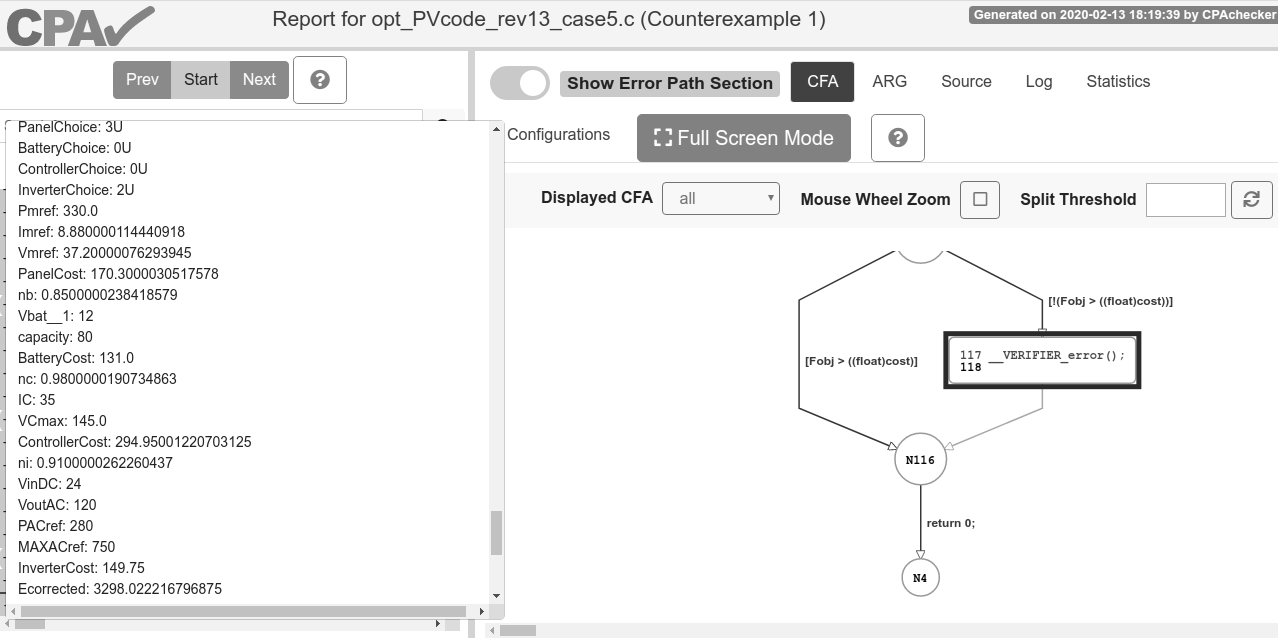
\includegraphics[width=0.47\textwidth]{CPA_opt_c5.png}}
\centering
\caption{Counterexample generated by CPAchecker after validation of case $5$.}
\label{fig:CPAoptc1}
\end{figure}

Here we used ESBMC in BMC incremental mode with Boolector; ESBMC was able to reach the optimal sizing of case studies $1$, $3$, $4$, $5$, and $6$ with a FAIL/ SAT response, varying from $36$ minutes to $10$ hours. ESBMC, with this configuration, was unable to obtain an optimal solution in cases $2$ and $7$. Case $2$ produced a \textit{time out}. Moreover, case $7$ resulted in a UNSAT result, i.e., ESBMC was unable to provide a feasible solution. However, this is not a bug, and it means that the available list of equipment can not produce a feasible solution that satisfies electrical compatibility or design requirements. This UNSAT situation was reached in less than one minute. These experimental results answer the \textit{EG2}.

HOMER Pro was able to evaluate six case studies (cases $1$, $2$, $4$, $5$, $6$, and $7$) under $30$ seconds; it was much faster than the proposed automated synthesis tool (cf.~\textit{EG3}). Case study $3$ could not be simulated since HOMER Pro does not have the battery autonomy adjustment feature, i.e., the tool always tries to feed the given load with electricity $365$ days/year. Some HOMER Pro drawbacks were also noted. (1) System equipment does not include an explicit charge controller. HOMER Pro includes a controller automatically to simulate the charge/discharge of batteries and to meet the load requirement. However, without costs or even with electrical characteristics such as maximum current and voltage, which are common during PV sizing. (2) HOMER Pro requires the inclusion of some battery specification to initiate optimization; however, it does not change the electrical specifications during simulation; the results presented are multiples of the original battery type suggested by the user. For example, it was started with an $83.4$ Ah lead-acid battery, and during simulation, HOMER Pro did not try to use other capacities or types. (3) HOMER Pro does not present the optimal solution in terms of connections of PV panel arrays, just the total in terms of power, i.e., it presents neither the models and the power of each PV panel nor the total of panels in series or parallel. The cost of every equipment item used in HOMER Pro is a US-based cost, without adaptation regardless of where the equipment is installed.

We have real PV systems deployed since June $2018$ in a riverside community in the State of Amazonas, Brazil, GPS coordinates 2$^{o}$44'50.0"S 60$^{o}$25'47.8"W, with demands of case studies $1$, $4$, $5$, and $6$, always with a $3$ $\times$ $325$ W ($3$S, total $975$ W) panels and $4$ $\times$ $220$ Ah ($2$S-$2$P $= 440$ Ah) lead-acid batteries.

%%%%%%%%%%%%%%%%%%%%%%%%%%%%%%%%%%%%%%%%%%%%%%%%%%%%%%%%%%%%%%%%%%%%
\subsection{Comparison Between Formal Synthesis and HOMER Pro}
%%%%%%%%%%%%%%%%%%%%%%%%%%%%%%%%%%%%%%%%%%%%%%%%%%%%%%%%%%%%%%%%%%%%

If we compare the formal synthesis results against those of HOMER Pro, we observed some distinct effects in terms of the technical solution and cost (cf. Table~\ref{tab1}). Concerning the performance, there exists a vast difference in favor of HOMER Pro that obtained the results in considerably less time: few seconds in the opposite of an average of $4$ hours for the automated synthesis technique. Particularly in the case of LCC, the cost varied from $11$\% to $44$\%, producing a higher estimation from the automated synthesis technique. However, considering that the cost of individual items of each database used to compose the optimal design is not the same among the tools, it is plausible to obtain distinct results.

On the one hand, concerning the PV panels sizing, the results presented by the automated synthesis were smaller in terms of power than the ones produced by the simulation tool. The difference varied from $19$\% to $65$\%. On the other hand, concerning the battery bank, the results were smaller in terms of HOMER Pro capacity. The difference was between $34$\% to $68$\%. The mathematical models are different and particular parameters can be tuned for each technique, and that can justify the difference, which was presented in all the case studies.

Those discrepancies are not easy to address without some real systems validation. However, we use the simulation software PVsyst to validate the optimal sizing produced, as shown in Table~\ref{tab2}. Note that PVsyst has a pre-sizing feature, which presents a minimum recommended sizing of PV panels and batteries (only) without using manufacturers' data or models for it. This feature was used as reference mainly with HOMER Pro, where there exists no equipment brands or models (only power and capacities specification). PVsyst was used with the field-deployed and the formal synthesis sizing solutions, where brands and models were simulated in PVsyst according to the sized system.
%
\begin{table*}
\centering
\caption{Optimal sizing validation with PVsyst.}
\label{tab2}
\begin{scriptsize}
\begin{tabular}{c|c|c|c|c}
\hline
\hline
CS & \makecell{PVsyst\\(pre-sizing)}& \makecell{Field\\deployed\\validation}& \makecell{Formal synthesis\\sizing\\validation}& \makecell{HOMER Pro\\sizing\\validation}\\
\hline
\hline
CS 1 & \makecell{P= 1,166 W\\B= 381 Ah\\(minimum)} & \makecell{Not correct sizing \\Avail. $<$ 95\%\\(91.06\%)} & \makecell{No error found \\100\% of avail.} & \makecell{No error found\\Panels oversized in 2.16 $\times$\\Batteries oversized in 1.39 $\times$}\\
\hline
CS 2 & \makecell{P= 1,482 W\\B= 478 Ah\\(minimum)} & \makecell{NA\\There exists no real PV system\\available for comparison} & \makecell{NA \\(TO result\\in Table~\ref{tab1})} & \makecell{No error found\\Panels oversized in 2.6 $\times$\\Batteries oversized in 1.74 $\times$}\\
\hline
CS 3 & \makecell{Not possible to \\simulate\\(autonomy $<$ 24h)} & \makecell{NA\\There exists no real PV system\\available for comparison} & \makecell{Only technique that\\produced solution} & \makecell{NA\\(autonomy $<$ 24h)}\\
\hline
CS 4 & \makecell{P= 1,078 W\\B= 354 Ah\\(minimum)} & \makecell{No error found \\95.76\% of avail.} & \makecell{No error found \\97.37\% of avail.} & \makecell{No error found\\Panels oversized in 2.24 $\times$\\Batteries oversized in 1.41 $\times$}\\
\hline
CS 5 & \makecell{P= 823 W\\B= 268 Ah\\(minimum)} & \makecell{No error found \\100\% of avail.} & \makecell{No error found \\100\% of avail.} & \makecell{No error found\\Panels oversized in 1.93 $\times$\\Batteries oversized in 1.56 $\times$}\\
\hline
CS 6 & \makecell{P= 1,299 W\\B= 421 Ah\\(minimum)} & \makecell{Not correct sizing \\Avail. $<$ 95\%\\(85.65\%)} & \makecell{No error found \\100\% of avail.} & \makecell{No error found\\Panels oversized in 2.42 $\times$\\Batteries oversized in 1.38 $\times$}\\
\hline
CS 7 & \makecell{P= 4,263 W\\B= 1,384 Ah\\(minimum)} & \makecell{NA\\There exists no real PV system\\available for comparison} & \makecell{NA \\(UNSAT result\\in Table~\ref{tab1})} & \makecell{No error found\\Panels oversized in 2.9 $\times$\\Batteries oversized in 1.99 $\times$}\\
\hline
\hline
\end{tabular}
\\Legend: CS = case study; NA = sizing not available for validation; B = batteries capacity; P = panels power; Avail.= Availability (expected of 95\% or greater as a design requirement).
\end{scriptsize}
\end{table*}

Each simulation with PVsyst took $4$ seconds. We were unable to validate the case study $3$ using PVsyst. The battery autonomy is less than 24 hours, and only the proposed synthesis technique can perform the optimal sizing (PVsyst and HOMER Pro are limited for a $24$ h minimum). Case studies $2$ and $7$ had only HOMER Pro sizing validation. There is no deployed equivalent system in the field, and the synthesis technique did not present a solution due to \textit{time out} and internal failures in the underlying verification engine. %(our technique presented a \textit{time out} in case study $2$ and an \textit{UNSAT} in the case study $7$).

Overall, those comparisons with our approach, the optimization software, and the deployed systems, with validation through simulation tool, show that the synthesis solution is sound and complete, which answers \textit{EG1} and {EG3}.

Concerning the cost (LCC) present by both tools, HOMER Pro does not use the real cost for PV systems deployed in Brazil; therefore, the optimal solution presented by HOMER Pro is notoriously cheaper than our technique. However, considering that the aim is to present an optimal PV sizing solution that is feasible and closer to the market prices, our technique is more indicated.

Besides that, HOMER Pro suggests a value in kW for the inverters that are very close to the maximum load of every case study, but it is not commercial. The proposed synthesis tool, however, presents inverters that are commercial and can be obtained off-the-shelf. Moreover, our synthesis approach considers surge power demand from the house, which is not viewed by HOMER Pro or PVsyst. This feature is a definite advantage of the formal synthesis method. HOMER Pro does not include charge controllers as a specific item of equipment in its mathematical model; only the synthesis tool presents a commercial controller and includes it during the cost analysis. The formal synthesis method, therefore, presents more reliable results than HOMER Pro.

In summary, our synthesis technique can present a solution that is far more detailed and closer to commercial conditions than the answer given by HOMER Pro. In particular, the automated synthesis method can provide all the details of every component of a PV system solution, with complete electrical information from the manufacturer datasheet, including the model of the component, nominal current, and voltage. In this respect, even the name of the manufacturer can be cited (in Table~\ref{tab1}, it was removed to avoid unauthorized advertising). Moreover, the validation through PVsyst simulation, using the PV sizing produced by HOMER Pro and our synthesis approach, shows that our results are feasible and not as oversized as HOMER Pro results, mainly concerning PV panels.

An optimal solution from a tool is not necessarily the same optimal from other tools, mainly when the database of equipment items (with different costs) is not the same \cite{Alsadi2018}. Therefore, the comparison must take this issue into account. 

%---------------------------------------------------------------------------
\subsection{Threats to validity} 
%---------------------------------------------------------------------------

We have reported a favorable assessment of the proposed method. Nevertheless, we have also identified four threats to the validity of our results that constitute future work. First, improvement of the power reliability analysis: to include loss of load probability or loss of power supply probability, which can make the study more accurate. Second, improvement of the system cost analysis by adding operational and maintenance costs to the adopted LCC analysis. Third, increase the equipment and manufacturers database: this will increase the optimization complexity, but the result will also allow improved sizing. Lastly, the underlying software verifiers employed here perform bit-precise verification based on the Floating-Point (FP) theory. We could use a real arithmetic strategy to tackle these equations; however, in this study, we have exploited the FP arithmetic, approximating the real one. 

%------------------------------------
\section{Conclusions} 
%------------------------------------

(VSTTE)Our novelty relies on a practical approach to pursue the optimal PV systems' optimal solution using contemporary formal methods. The use of formal synthesis to design PV systems has no precedent in literature; we show that our approach results, using seven case studies, are promising. Our synthesis tool can present a solution that is far more detailed and closer to commercial reality than the solution given by the commercial tool. The battery autonomy feature, together with the details of every component of a PV system solution, is advantageous for our synthesis approach; these details are essential for the PV system owner. The industry demands proximity between the result presented by optimization tools and the items of equipment for solar systems available on the market. 

Our synthesis technique was developed and used open-source software verifiers and the environment, in contrast to the optimization and simulation tools used in this work. We have also observed that state-of-the-art software verifiers are doing an excellent job of solving hard verification conditions based on the underlying SAT/SMT solvers. Lastly, the use of data from real deployed systems in Brazil and the validation through PVsyst was essential to validate the comparison. We have shown that our technique has a promising result for PV system sizing optimization. Our focus for future work consists of improving the search mechanism used in the {\sc Verify} phase of our synthesis technique to speed up the overall time. We plan to use parallel binary search~\cite{TrindadeDJISC17} or even a solver that is specific to perform optimization with model checking as $\nu Z$~\cite{BjornerPF15}.

(IEEETOSE) We have described and evaluated an automated synthesis method to obtain the optimal size of the PV system using software model checking. The focus was on the synthesis method to obtain the optimal solution based on formal methods, which can cover better the design-space as opposed to simulation tools. We have considered seven case studies from PV systems in two different sites of the Amazonas State in Brazil, ranging from $253$\,W to $1,586$\,W peak. One state-of-art verification engine was considered (ESBMC), in addition to a specialized off-the-shelf optimization tool (HOMER Pro) to compare the results. The validation through PVsyst was essential to perform the comparison. The paper produced methodological research with innovative value regarding the first use of automated synthesis for optimal sizing of solar PV systems.

In summary, our synthesis tool is capable of presenting a solution, which is far detailed and close to the commercial reality than the solution presented by HOMER Pro. In particular, our method can provide all the details of every component of a PV system solution, with complete electrical details from the datasheet of manufacturers, including the model of the component, nominal current, and voltage. We also cover the charge controller, which is unavailable in HOMER Pro. Note that our automated synthesis tool took longer to find the optimal solution than HOMER Pro; however, the presented solution is sound and complete; it also provides a list of equipment to be bought from manufacturers. Moreover, we extended the CEGIS synthesis method and implemented this extension within our proposed formal synthesis tool, which allows the optimization of stand-alone PV systems with the best compromise between power reliability and system cost analysis. For future work, we plan to improve the power reliability analysis to address the restriction to only allow automated synthesis of riverside communities in the Amazonas state (Brazil) and to validate some cases with the deployment of real PV systems in isolated communities.


%
%\appendices
%\section{Proof of the First Zonklar Equation}
%Appendix one text goes here.
% you can choose not to have a title for an appendix
% if you want by leaving the argument blank
%\section{}
%Appendix two text goes here.
% use section* for acknowledgment
\section*{Acknowledgments}
This study was financed in part by the Coordenação de Aperfeiçoamento de Pessoal de Nível Superior - Brazil (CAPES) - Finance Code 001.
% Can use something like this to put references on a page
% by themselves when using endfloat and the captionsoff option.
%\ifCLASSOPTIONcaptionsoff
%  \newpage
%\fi
% trigger a \newpage just before the given reference
% number - used to balance the columns on the last page
% adjust value as needed - may need to be readjusted if
% the document is modified later
%\IEEEtriggeratref{8}
% The "triggered" command can be changed if desired:
%\IEEEtriggercmd{\enlargethispage{-5in}}
% references section
% can use a bibliography generated by BibTeX as a .bbl file
% BibTeX documentation can be easily obtained at:
% http://mirror.ctan.org/biblio/bibtex/contrib/doc/
% The IEEEtran BibTeX style support page is at:
% http://www.michaelshell.org/tex/ieeetran/bibtex/
\bibliographystyle{IEEEtran}
% argument is your BibTeX string definitions and bibliography database(s)
\bibliography{references}{}
%
% <OR> manually copy in the resultant .bbl file
% set second argument of \begin to the number of references
% (used to reserve space for the reference number labels box)
%
%\begin{thebibliography}{1}
%\bibitem{IEEEhowto:kopka}
%H.~Kopka and P.~W. Daly, \emph{A Guide to \LaTeX}, 3rd~ed.\hskip 1em plus
%  0.5em minus 0.4em\relax Harlow, England: Addison-Wesley, 1999.
%\end{thebibliography}
%
%%%%%%%%%%%%%% biography section
% 
% If you have an EPS/PDF photo (graphicx package needed) extra braces are
% needed around the contents of the optional argument to biography to prevent
% the LaTeX parser from getting confused when it sees the complicated
% \includegraphics command within an optional argument. (You could create
% your own custom macro containing the \includegraphics command to make things
% simpler here.)
%\begin{IEEEbiography}[{\includegraphics[width=1in,height=1.25in,clip,keepaspectratio]{mshell}}]{Michael Shell}
% or if you just want to reserve a space for a photo:
\begin{IEEEbiography}
    [{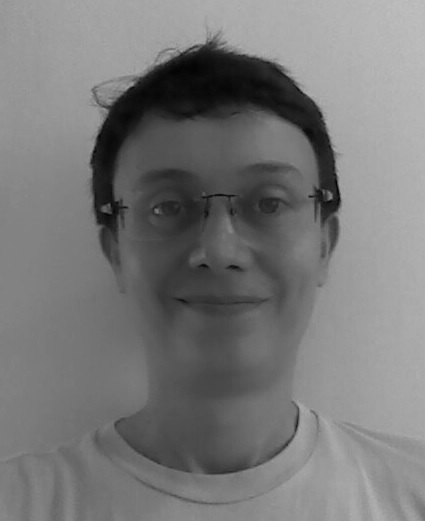
\includegraphics[width=1in,height=1.25in,clip,keepaspectratio]{alessandro3por4_2}}]{Alessandro Trindade}
received his PhD in Computing, BSc and MSc in Electrical Engineering from the Federal University of Amazonas (UFAM) in 2020, 1995 and 2015, respectively. Currently, he holds an Adjunct Professor position in the Electricity Department from UFAM. Prior to joining UFAM, he worked 4 years as Consultant of renewable energy to the Amazonas State Electric Utility and to the Inter-American Institute for Cooperation on Agriculture (IICA); he also worked for 12 years as R\&D and project manager at a non-profit foundation. His interest is in renewable energy, automated verification, and model checking.
\end{IEEEbiography}
%
%\begin{IEEEbiographynophoto}{Alessandro Trindade}
%received his BSc and MSc in Electrical Engineering from the Federal University of Amazonas (UFAM) in 1995 and 2015, respectively. Currently, he is pursuing his PhD in the Postgraduate Program in Informatics (PPGI) at UFAM, and holds an Assistant Professor position in the Electricity Department from UFAM. Prior to joining UFAM, he worked 4 years as Consultant of renewable energy to the State Electric Utility and to the Inter-American Institute for Cooperation on Agriculture (IICA); he also worked for 12 years as R\&D and project manager at a non-profit foundation (Centre of Analysis, Research and Innovation Technology Foundation). His interest is in renewable energy, automated verification, and model checking.
%\end{IEEEbiographynophoto}
%
\begin{IEEEbiography}
    [{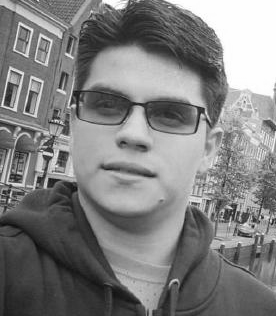
\includegraphics[width=1in,height=1.25in,clip,keepaspectratio]{edilsonphoto}}]{Edilson Galvao}
received his BSc in Computer Engineering from the Federal University of Amazonas (UFAM) in ?????. Currently, he pursues MSc in CS at UFAM. text here. His interest is in automated verification, and model checking.
\end{IEEEbiography}

\begin{IEEEbiography}
    [{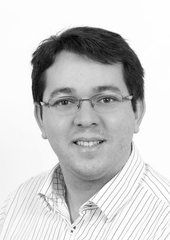
\includegraphics[width=1in,height=1.25in,clip,keepaspectratio]{lucas3por4}}]{Lucas Cordeiro}
received his Ph.D. degree in Computer Science in 2011 from the University of Southampton, UK. Currently, he is a Senior Lecturer in the School of Computer Science at the University of Manchester, and leads the Systems and Software Verification laboratory. He is also a collaborator in the Postgraduate Program in Electrical Engineering and Informatics at the Federal University of Amazonas (UFAM), Brazil. Prior to joining the University of Manchester, he worked as a researcher at Oxford University / Diffblue and as an adjunct professor at UFAM; he also worked for 4 years as software engineer at industry. His work focuses on software model checking, automated testing, program synthesis, and embedded \& cyber-physical systems.
\end{IEEEbiography}
% insert where needed to balance the two columns on the last page with
% biographies
%\newpage
%\begin{IEEEbiographynophoto}{Jane Doe}
%Biography text here.
%\end{IEEEbiographynophoto}
% You can push biographies down or up by placing
% a \vfill before or after them. The appropriate
% use of \vfill depends on what kind of text is
% on the last page and whether or not the columns
% are being equalized.
%\vfill
% Can be used to pull up biographies so that the bottom of the last one
% is flush with the other column.
%\enlargethispage{-5in}
% that's all folks
\end{document}
